\chapter{Dynamic Instrumentation Using Code Analysis And Transformation For Detailed GPU Communication Analysis}
This chapter describes in detail how the instrumentation works and will do so in the same order of steps as how an application is processed to generate traces.
First, the original application is instrumented on AST and LLVM IR level for tracing, then the data is generated on the GPU during the execution and transported to the host where it is stored in the trace file.

As libraries present external code not in source or LLVM IR, code using libraries can not be reliably instrumented.

Figure \ref{compilestack} shows the necessary steps to add tracing to an application. The first step performs source-to-source compilation that augments the following kinds of statements in the original source with instructions required
for tracing.

These augmentations have to be performed for each file that contains either of the above statements individually because the process generated new files
rather than overwriting the original source files. More details on the matter in section \ref{sec:impl:clang}


CUDA application have a heterogeneous memory hierarchy, offering different address spaces, which offer varying characteristics to the user.

\begin{itemize}
	\item \textbf{Shared Memory Space} is private to each CTA. Low access latency, low capacity. Located on each Shared Multiprocessor.
	\item \textbf{Global Memory Space} is the primary memory of a GPU. Shared by all CTAs. High access latency, high bandwidth, highest capacity on GPU.
	\item \textbf{Texture Memory} shared ROM for all CTAs. All reads are cached.
	\item  ...
\end{itemize}



The next step is the introduction to 

Then explain how the tracing is introduced into the application
\begin{enumerate}
	\item Generate object files from augmented source files and insert tracing with LLVM Plugin:
	\item Linking
\end{enumerate}


\section{Source to Source Compilation in CLang}\label{sec:impl:clang}
The first instrumentation step extends the original source code with the information for the buffers used during the trace, specifically the items listed below.
\begin{itemize}
	\item Kernel Declarations
	\item Kernel Definitions
	\item Kernel calls
	\item \verb|__device__| function declaration
	\item \verb|__device__| function definitions
	\item \verb|__device__| Function calls inside a Kernel
\end{itemize}


\begin{itemize}
	\item User has to know which files need augmentation
	\item Augmentation of one file at a time, since out-of-place code transformation is performed
	\item Working in Clang AST
	\item Find all places in the code that need Augmentation:
	\begin{enumerate}
		\item Kernel Definition: Add set of arguments used for tracing
		\item Kernel Calls: Add arguments used for tracing
		\item Include File offering the tracing utils
	\end{enumerate}
\end{itemize}
\section{Code Transformation in LLVM}
Instrumenting the application to generate trace data for global memory operations on the GPU happens inside a LLVM IR optimisation pass. The original source is analysed and instrumented at the locations of loads, stores and atomic operations targeting global memory, so that during the execution data is generated.

Global memory is the only address space of a CUDA application, that allows communication with other CTAs and so only memory operations using this address space needs instrumentation. CLang performs lowering of all memory access operations during the generation of LLVM IR and in the process eliminates the address space information
at location of the memory operation. An example for the lowering is displayed in listing \ref{lowering}, showing
that the information is 'casted' away by the IR. PTX however, does not need address space information for a memory operation since it can be resolved dynamically during runtime at the cost of a minor performance decrease[ref here...]. And therefore the loss of this information is not a concern for building a correct application. For the tracing process however, we need to have this information to prevent the generation of trace data for parts of the address space that are not interesting for this work.

\begin{figure}
	\begin{lstlisting}[style=C]

C:	data[id] = 1
	==========================
LLVM: addrspacecast
	  gep
	  bitcast
	  store
	\end{lstlisting}
	\caption{Example for address space lowering in LLVM IR}
	\label{lowering}
\end{figure}

While an experimental LLVM optimizer pass exists, which tries to infer the address space by analysing the steps
that have been introduced by the lowering, it works on a function scope and only performs a 'may-analysis', which is not sufficient for our purposes. Address space information  might not be existing in the function argument because of lowering previous to the function call. And due to the pass' function scope, information on the calling context is not available.
Therefore a 'must-analysis' is performed, that generates definitive information, whether a memory access targets
global memory or not. If generating this information is not possible, the pass fails. The reason for an unsuccessful execution is  explained in section \ref{pa}, after more details of the actual analysis have been
explained.

While the developed pass tries to cover as much code as possible, it can only operate in the boundaries of 
LLVM. The pass is designed as a 'Module'-pass which provides a context for the whole compilation unit. Code beyond this compilation unit can not be instrumented during this run of the pass.

\subsection{Address Space Analysis}\label{pa}
The basic principle of this analysis rests on the observation, that there is only a limited number of sources in
a kernel, where a global address space pointer can be obtained from in the first place.
\begin{itemize}
	\item Direkt kernel parameter
	\item indirekt kernel paramete (struct etc.)
	\item global variables
	\item Pointer Type load from global memory
\end{itemize}
Collecting base pointers form all these sources provides starting points for a sparse analysis of the program,
because only memory operations that are part of def-use chains rooting in these base pointers, can be a candidate for instrumentation.


 Proof Global Memory "origin" of Pointer used in Memory operations (Load, Store, Atomics): Context Sensitive, Spase Flow Analysis in SSA, 3 Element Lattice Problemspace, Monotonic Transfer function, Pathological Cases (PhiNodes/Certain Functions)
\subsection{Versioning}\label{vers}
Replicate Device Functions with ambiguous memory spaces
\subsection{Instrumentation}\label{vers}
Code Transformation: Insert Instructions used for tracing

\section{Tracing Process}
	Many applications have non-deterministic executions, for example no predetermined number of kernel calls because of varying input data. Examples are graph algorithms depending on the underlying graph's structure or numerical solvers, which iterate until a
	convergence condition is reached by the residual. Because of this, a static buffer that is filled up once and is cleared at the end of the application does no suffice for reliable and dynamic tracing.
	
	Therefore a producer-consumer for the generated trace data between GPU and host is used that ensures the application never runs out of buffer space for the tracing data. The GPU generates the data and the host evacuates full buffers, storing the data.
	The buffer containing the generated data is host-mapped memory, which is separated into several bins. The bins are used to reduce
	pressure on the memory system that is generated by the atomic index accesses of the producer-consumer setup. The number of bins 
	is always a $2^n$ and a scheduled CTA uses the  $n$ least significant bits of the SM's ID it is scheduled on, to select a bin. Therefore the number of bins should be selected as the closest power of two, to the number of SMs.

	Writing the data to the disk after they have been cleared from the buffer by the consumer, showed to be a performance critical aspect during the trace. Per default, Linux directs \verb|writes()| to a page cache, that is evicted periodically. Smaller, periodic writes to the disk proved to be more efficient in this case, because it gives the kernel time to evict the page cache while the consumer looks for
	the next full buffer. Therefore, smaller bins, around (64Kbyte to 1Mybte), showed better performance than larger bins.
	
	\subsection{On-Device Producer}
\begin{figure}[t]
	\centering
	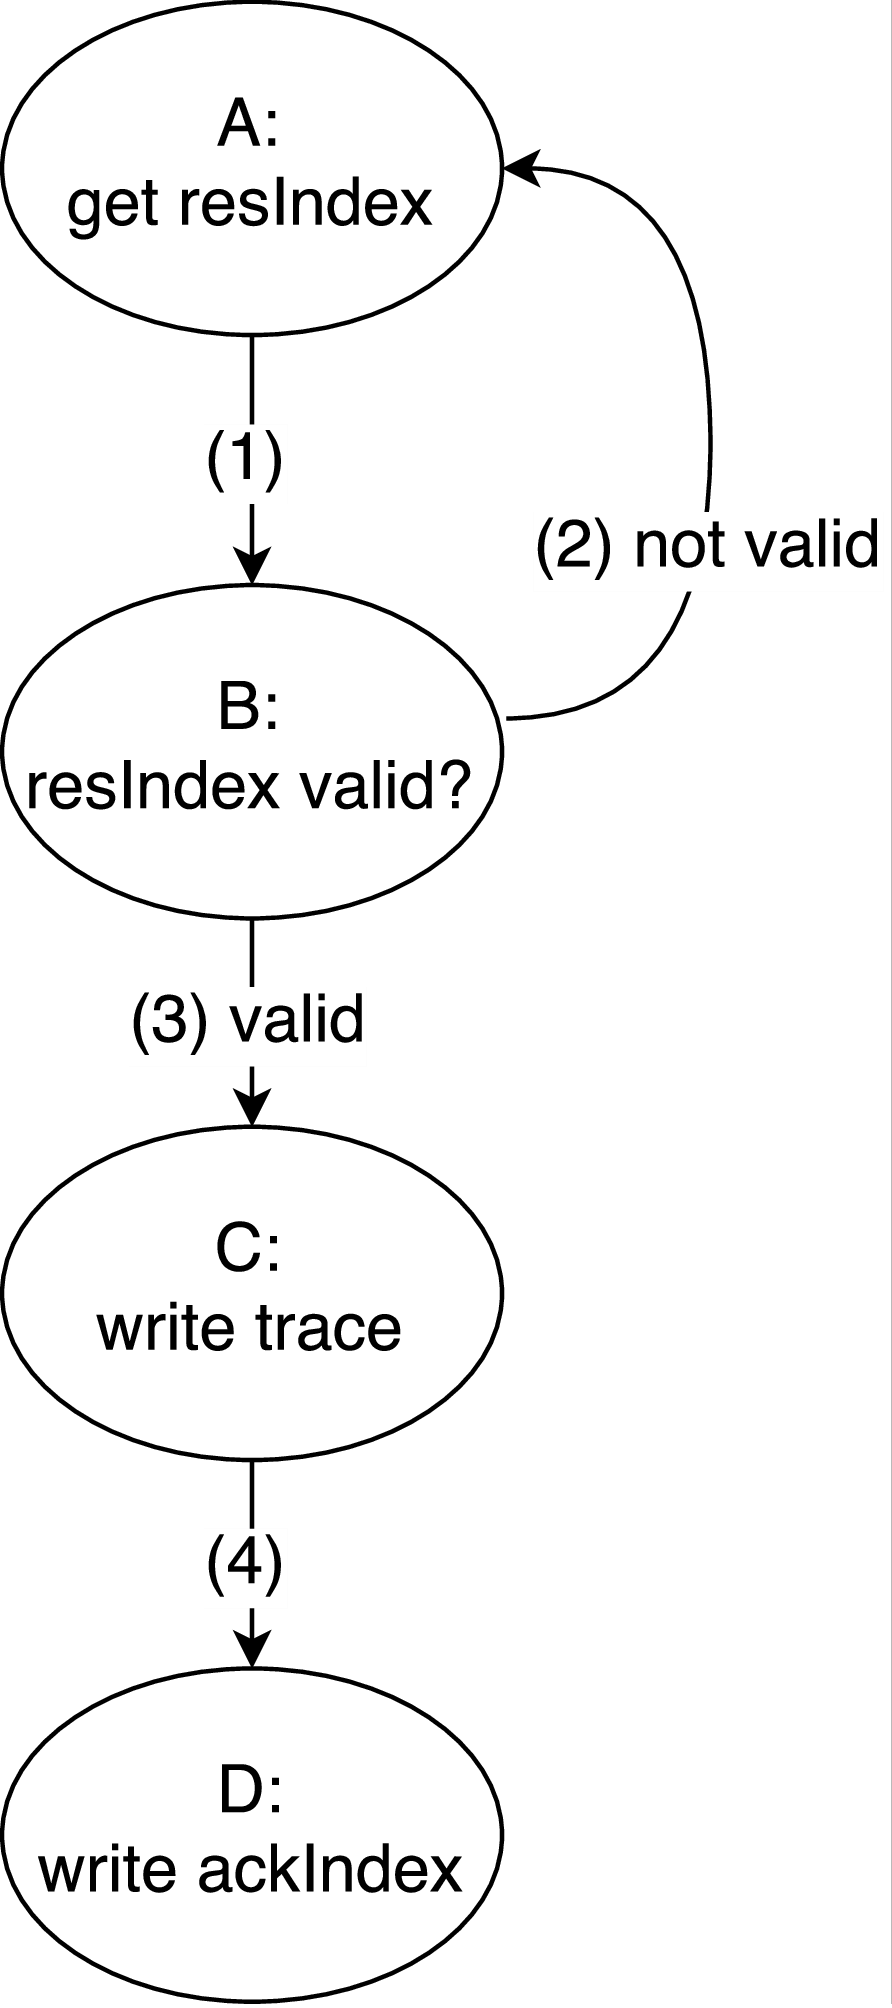
\includegraphics[width=0.3\textwidth]{warp-scope-cfg}
	\caption{Producer CFG}
\label{wscfg}
\end{figure}	
	This section focusses on the producer that is running on the device, making sure that data is only written if there space left
	in a buffer. The producer-consumer setup uses a head and a tail index to handle reservation of buffer space and write acknowledgements to signal that the write has completed. Code sample \ref{prod-cons} shows the pseudo-algorithm that is performed by the producer. First the required buffer space is reserved for writing by incrementing the reservation index
	by the number of required slots (line 1). Then the data generated by the trace is
	written to the buffer (line 2) and the write acknowledgement is incremented by the same number of buffer slots (line 3).
\begin{figure}
	\begin{lstlisting}[style=C]
while((ackIndex > maxIndex) or (id = atomicAdd(resIndex, increment) > maxIndex));
buffer[id] = traceData;
atomicAdd(ackIndex, increment);
\end{lstlisting}
	\caption{Device Producer, naive approach}
	\label{prod-cons}
\end{figure}

	
	This is implemented on a warp scope, which means either the whole warp continues or waits, to prevents deadlocks during indices fetching.
	A deadlock can occur because of how GPUs manage branch divergence inside a warp. If the instruction stream of a warp branches, all member threads of this warp execute both branches, and the group of members that should not be executing this part of the code is masked out. After all branches completed execution, the combined execution of both groups continues.
	
	A deadlock can occur, if each thread fetches it's \verb|resIndex| individually and there is not enough available buffer space for all threads inside the warp. Referring to figure \ref{wscfg} now, all threads will execute edge (1) leading from (A) to (B) by fetching \verb|resIndex|. If all threads get a valid index (B), the warp will not branch and the trace can complete successfully.
	If the check in (B) fails for one or more threads in the warp, a branch is created. The branch without valid IDs will 
	use edge (2), returning to node (A) and retry fetching a valid \verb|resIndex|. The branch with valid \verb|resIndex|
	has to wait with progressing on edge (3) until the group without valid \verb|resIndex| is also ready to continue on edge (3).
	But because the warp can not progress over edge (3) to and C and from there over (4) to D, until all threads have a valid \verb|resIndex|, the threads in the warp that already have a valid \verb|resIndex| can not reach node D write \verb|ackIndex|, which would lead to a evacuation of the buffer on by the host and a reset of the \verb|achIndex| and \verb|resIndex|. As a result of this, a deadlock occurs because one group of threads waits for a resource that can not be released by the other group
	of threads due to the warp execution model.
	
	This can be resolved by handling reservation and write acknowledgement on a warp level. One thread makes the reservation and write the acknowledgement for all threads inside the warp. Now either the whole warp can finish the trace or the whole warp stalls. This way we can use the warp execution model for our purposes, because one thread that waits for the IDs can stall the whole warp with an if branch and no other means of synchronization. This is implemented by using CUDA warp intrinsics, which offer efficient communication inside of warps.
\begin{figure}[t]
	\begin{lstlisting}[style=C]
active   = __ballot(1); // get bitmap of active threads 
nActive  = __popc(active); // get count of active threads
lowest   = __ffs(active)-1; // check which thread has to perform sync
rlane_id = __rlaneid(active, lane_id); // each thread gets its relative Lane id, based on number of active threads
	
if (lane_id == lowest)
	while( ackIndex >= maxIndex-maxWarpWrite 
		|| (id = atomicAdd(resIndex, nActive)) >= maxIndex-maxWarpWrite
	);
// Warp stalls here until all branch is completed

idx = __shfl(id, lowest) + rlane_id; // distribute id
buffer[id] = traceData;
if (lane_id == lowest )
	atomicAdd(ackIndex, n_active);
	\end{lstlisting}
	\caption{Device Producer, warp scope}
	\label{prod-cons-warp}	
\end{figure}
	Little extra code is needed shift everything to a warp-scope management, as seen in Figure \ref{prod-cons-warp}. Because it is possible that a trace occurs on a point during the execution, where the warp is already branched we have to make sure
	that the indexes are managed correctly and only the currently active threads participate in the trace. The warp intrinsics \verb|__ballot|, \verb|__popc| and \verb|__ffs| are used to determine how many threads are active, and which one has to perform the atomic operations to handle
	the producer synchronization. Then \verb|__rlaneid()|, which is user code, calculates the relative lane id for each warp. 
	
	While the lowest thread fetches the id for the buffer using \verb|atomicAdd|, the whole warp stalls at the end of the if clause because of the warp execution model. Once a valid id is fetched, it is distributed among all threads using the \verb|__shfl| intrinsic. 	Then the trace is written and the lowest thread increments the write acknowledgement by the number it increased the reservation.
	
	Notice that in this case, the conditions for fetching the id now takes into account that data is written in blocks and has to check if there is still space left for one complete block. 
	
	Assuming a warp is fully populated warp at the moment a trace happens and thus always reserve enough buffer space for a whole warp can create gaps in the trace data. To prevent old data from lingering, the buffer would need to be wiped after every evacuation of the
	generated trace data. Additionally, these gaps would require additional handling in the analysis of the data.
	Therefore, this more complex approach of handling the consumer was chosen, which only reserved as much space as required.

	
	\subsection{Host Consumer}
	The consuming thread on the host side is much simpler. A single thread is iterating over all bins in the buffer, checking if the
	\verb|ackIndex| is at the threshold for evacuation. This threshold is reached if there is not enough space for a complete warp to
	write a trace.
	The buffer is evacuated by writing the data into a file handle and \verb|resIndex| and \verb|ackIndex| reset to the beginning of the buffer.
%	
%	...
%
%\begin{itemize}
%	\item General Tracing Setup
%	\item Producing Data on the Device: Handling Indices on a Warp Scope
%	\item Consuming data on the host side
%	\item Handling Streams
%\end{itemize}
%

